
\section{Conversão - norma IEEE 754/2008} \label{sec:conversão}

\begin{enumerate}
	% *****************************************************************
\item Represente os números a seguir nos formatos abaixo solicitados: 
{\bf 81, 66.25, -0.625, 0.533203125}.
    \begin{enumerate}
        \item Binário convencional;
        \item Binário em ponto flutuante;
        \item Cadeia de 32 bits em precisão simples conforme a norma IEEE--754.
        \item Cadeia de 64 bits em precisão dupla conforme a norma IEEE--754.
    \end{enumerate}
    
\item Faça um {\it script} que receba um número decimal {\bf positivo} e converta-o para:
    \begin{enumerate}
        \item Binário convencional;
        \item Binário em ponto flutuante;
        \item Cadeia de 32 bits em precisão simples conforme a norma IEEE--754;
        \item Cadeia de 64 bits em precisão dupla conforme a norma IEEE--754;
    \end{enumerate}
    
\item Faça um {\it script} que receba um número decimal {\bf negativo} e converta-o para:
	\begin{enumerate}
        \item Binário convencional;
        \item Binário em ponto flutuante;
        \item Cadeia de 32 bits em precisão simples conforme a norma IEEE--754;
        \item Cadeia de 64 bits em precisão dupla conforme a norma IEEE--754;
    \end{enumerate}
    
\item Faça um {\it script} que receba um número decimal com {\bf mantissa} (parte não inteira) e converta-o para:
\begin{enumerate}
        \item Binário convencional;
        \item Binário em ponto flutuante;
        \item Cadeia de 32 bits em precisão simples conforme a norma IEEE--754;
        \item Cadeia de 64 bits em precisão dupla conforme a norma IEEE--754;
\end{enumerate}

\item Utilizando POO, ajuste o {\it script} da questão anterior para receber o número decimal em quaisquer modos supracitados e convertê-lo para as saídas 
    anteriormente exploradas.
    
%=======================================================================
\section{Diferenciação Numérica} \label{sec:diferenciação}

\item  Considere a função $f(x) = x^3$. Calcule numericamente a derivada primeira no ponto $x = 3$ aplicando as
fórmulas de diferenças finitas progressiva, regressiva e central, utilizando:
\begin{itemize}
    \item os pontos x = 2, x = 3 e x = 4.
    \item os pontos x = 2,75, x = 3 e x = 3,25.
\end{itemize} 
Compare os resultados com a derivada exata (analítica) e expresse os erros relativo e absoluto.


\item Considere a função $f(x) = \ln(x)$. 
Utilize a fórmula de diferença progressiva de primeira ordem para aproximar $f'(1)$ com $h = 0{,}1$. 
Compare com o valor exato da derivada e calcule o erro absoluto.

\item Dada a função $f(x) = e^{-x}$, utilize a fórmula de diferença centrada de segunda ordem para estimar $f'(0)$ com $h = 0{,}05$. 
Analise a ordem do erro de truncamento.

\item A tabela abaixo fornece valores experimentais de uma função:

\[
\begin{array}{c|c}
x & f(x) \\
\hline
1{,}0 & 2{,}7183 \\
1{,}1 & 3{,}0042 \\
1{,}2 & 3{,}3201 \\
\end{array}
\]

Utilize a fórmula de diferença regressiva para estimar $f'(1{,}2)$.

\item Considere a função $f(x) = x^3 - 2x + 1$. 
Utilize:
\begin{itemize}
\item diferença progressiva,
\item diferença regressiva,
\item diferença centrada,
\end{itemize}
para estimar $f'(2)$ com $h = 0{,}1$. 
Compare os resultados e identifique qual método apresenta menor erro.

\item A função $f(x) = \sin(x)$ é avaliada numericamente. 
Utilize a fórmula de três pontos centrada para aproximar $f''(\pi/4)$ com $h = 0{,}01$. 
Compare com o valor analítico da segunda derivada.

\item Em um experimento de vibração, um bloco de massa $m$ é preso
 a uma mola com dureza $k$ e a um amortecedor
com coeficiente de amortecimento $c$, conforme mostrado
na Figura \ref{fig:sistema_massa_mola}. 
\begin{figure}[!h]
    \centering
    \caption{Sistema massa-mola}
    \label{fig:sistema_massa_mola}
    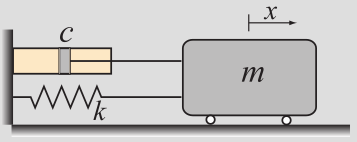
\includegraphics[scale=0.5]{figuras/SistemaMassaMola}\\
    \footnotesize{Fonte: adaptado de \citep{gilat2008}}
\end{figure}

Para que o experimento tenha início, o bloco é retirado da posição de equilíbrio e solto. 
A posição do bloco em função do tempo é gravada em uma freqüência
de $5 Hz$ (5 vezes por segundo). 
% Os dados gravados nos primeiros $10$ s são mostrados na Figura.
Os dados no intervalo $4 \le t \le 8$ s são dados a seguir.
\[
\begin{aligned}
t = \{&4.0,\, 4.2,\, 4.4,\, 4.6,\, 4.8,\, 5.0,\, 5.2,\, 5.4,\, 5.6,\, 5.8,\,6.0,\, 6.2,\, 6.4,\, 6.6,\, 6.8,\, 7.0,\, 7.2,\, 7.4
\\ & 7.6,\, 7.8,\, 8.0\}
\end{aligned}
\]
\[
\begin{aligned}
x = \{&-5.87,\, -4.23,\, -2.55,\, -0.89,\, 0.67,\, 2.09,\, 3.31,\, 4.31,\, 5.06,\,5.50,\, 5.77,\, 5.52,\, 5.08\\
& 4.46,\, 3.72,\, 2.88,\, 2.00,\, 1.10,\, 0.23,\, -0.59\}
\end{aligned}
\]
Com base nos dados deste experimento calcule:
    \begin{enumerate}
        \item A velocidade do bloco é a derivada da posição em
    relação ao tempo. Utilize a fórmula de diferença finita central para calcular a velocidade nos tempos $t = 5$s e $t = 6$ s.
        \item Escreva um {\it script} que calcule a derivada de uma função descrita por um conjunto de pontos. 
        Denomine a função de $dx=derivada(x,y)$,em que $x$ e $y$ são vetores com as coordenadas dos pontos, e $dx$ é um vetor com a derivada $dy/dx$ em
    cada ponto. A função deve calcular a derivada no primeiro e no último ponto usando as fórmulas de diferenças finitas progressiva e regressiva, respectivamente, 
    e usando a fórmula de diferença finita central nos demais pontos. 
        \item Utilize os pontos fornecidos para calcular a velocidade do bloco em $4 \le t \le 8$s. 
        \item Calcule a aceleração do bloco a partir da diferenciação da velocidade. 
        \item Trace um gráfico contendo deslocamento, velocidade e aceleração versus tempo para $4 \le t \le 8$s.
    \end{enumerate}


\item Em um ensaio de tração uniaxial de um aço, foram obtidos os seguintes dados experimentais de tensão ($\sigma$) 
em função da deformação ($\varepsilon$):
\[
\begin{array}{c|c}
\varepsilon & \sigma \; (\text{MPa}) \\
\hline
0.0000 &   0.0 \\
0.0002 &  42.0 \\
0.0004 &  85.0 \\
0.0006 & 128.0 \\
0.0008 & 170.0 \\
0.0010 & 210.0 \\
0.0012 & 250.0 \\
0.0014 & 295.0 \\
0.0016 & 340.0 \\
0.0018 & 380.0 \\
0.0020 & 420.0 \\
0.0022 & 455.0 \\
0.0024 & 485.0 \\
0.0026 & 510.0 \\
0.0028 & 535.0 \\
0.0030 & 555.0 \\
\end{array}
\]

\begin{enumerate}
\item Utilize a fórmula de diferença centrada para estimar numericamente o módulo de elasticidade tangente
 $ E_i = \dfrac{d\sigma}{d\varepsilon}$ nos pontos internos da tabela.

\item Utilize fórmulas de diferença progressiva e regressiva para estimar $E$ nos pontos extremos.

\item Com base nos valores obtidos, identifique o intervalo de deformação no qual o material apresenta comportamento aproximadamente linear.

\item Estime o módulo de elasticidade médio $E$ do material na região elástica e compare com o valor típico para o aço ($E \approx 200$ GPa).

\item Discuta a influência da discretização dos dados na precisão da estimativa de $E$, 
considerando erros de truncamento e possíveis ruídos experimentais.

\end{enumerate}


\item Utilizando POO, ajuste o \textit{script} da questão anterior para receber os vetores de $\sigma, \epsilon$ e retornar a análise gráfica conforme realizado
na questão acima.


\item Um sistema de aquisição de dados registrou medições discretas de tensão $V(t)$ e corrente $I(t)$ de uma carga elétrica ao longo do tempo. Os dados obtidos são apresentados na tabela a seguir:

\[
\begin{array}{c|c|c}
t \; (\text{s}) & V \; (\text{V}) & I \; (\text{A}) \\
\hline
0.0 & 220.000 & 0.52 \\
0.5 & 220.495 & 0.61 \\
1.0 & 220.958 & 0.68 \\
1.5 & 221.363 & 0.74 \\
2.0 & 221.683 & 0.79 \\
2.5 & 221.898 & 0.76 \\
3.0 & 221.995 & 0.70 \\
3.5 & 221.968 & 0.99 \\
4.0 & 221.818 & 1.49 \\
4.5 & 221.556 & 0.36 \\
5.0 & 221.197 & 0.28 \\
5.5 & 220.763 & 0.19 \\
6.0 & 220.282 & 1.14 \\
6.5 & 219.784 & 1.15 \\
7.0 & 219.298 & 0.18 \\
7.5 & 218.856 & 1.27 \\
8.0 & 218.486 & 0.38 \\
8.5 & 218.212 & 0.47 \\
9.0 & 218.045 & 0.59 \\
9.5 & 217.990 & 0.71 \\
10.0 & 218.082 & 0.78 \\
\end{array}
\]

Com base nesses dados, responda:

\begin{enumerate}

\item Calcule a potência instantânea $P(t_i)$ em cada ponto da tabela utilizando:
\[
P(t_i) = V(t_i)\,I(t_i).
\]

\item Utilize as seguintes aproximações de diferenças finitas para estimar numericamente a derivada da potência:

\begin{itemize}
\item Diferença progressiva:
\[
\left.\frac{dP}{dt}\right|_{t_i} \approx \frac{P_{i+1} - P_i}{t_{i+1} - t_i}
\]

\item Diferença regressiva:
\[
\left.\frac{dP}{dt}\right|_{t_i} \approx \frac{P_i - P_{i-1}}{t_i - t_{i-1}}
\]

\item Diferença centrada:
\[
\left.\frac{dP}{dt}\right|_{t_i} \approx \frac{P_{i+1} - P_{i-1}}{t_{i+1} - t_{i-1}}
\]
\end{itemize}

\item Compare os três métodos de diferenciação numérica e discuta suas diferenças em termos de precisão e comportamento nas extremidades do intervalo.

\item Construa os seguintes gráficos em um arranjo $2\times 2$:
\begin{itemize}
\item $V(t)$ em função do tempo;
\item $I(t)$ em função do tempo;
\item $P(t)$ em função do tempo;
\item comparação entre $\dfrac{dP}{dt}$ obtido pelos três métodos.
\end{itemize}

\item Determine os instantes de tempo em que ocorrem:
\begin{itemize}
\item o maior aumento de potência;
\item a maior queda de potência.
\end{itemize}

\item Com base nos resultados obtidos, interprete o comportamento dinâmico da carga, identificando possíveis transientes e variações abruptas de consumo.

\item Discuta a influência do passo de amostragem $\Delta t$ na precisão das derivadas numéricas e na representação gráfica dos dados.

\end{enumerate}

\item Utilizando POO, ajuste o \textit{script} da questão anterior para receber os vetores de $I,V,t$ e retornar a análise gráfica conforme realizado
na questão acima.

\section{Integração Numérica}\label{sec:integração}
\item Implemente um \textit{script} que realize a aproximação da integral definida utilizando o método do trapézio simples.

Aplique a função para calcular:
\[
\int_{0}^{2} (x^2 + 1)\,dx
\]

Determine também o erro absoluto em relação ao valor analítico da integral.

\item Implemente o método do trapézio composto e utilize-o para aproximar a integral:
\[
\int_{0}^{1} e^x \, dx
\]

Considere os valores $n = 4, 8, 16, 32, 48$ subintervalos. Apresente os resultados em forma de tabela e analise a convergência do método.

\item Implemente o método de Simpson 1/3, garantindo que o número de subintervalos $n$ seja par.

Utilize o método para calcular:
\[
\int_{0}^{2} \ln(x+1)\,dx
\]

Compare os resultados com aqueles obtidos pelo método do trapézio composto utilizando o mesmo número de subintervalos.

\item Para a integral:
\[
\int_{0}^{\pi} \sin(x)\,dx
\]

Implemente e compare os seguintes métodos:
\begin{itemize}
    \item Método do ponto médio
    \item Método do trapézio
    \item Método de Simpson 1/3
\end{itemize}

Utilize $n = 4, 10, 50$ subintervalos. Construa um gráfico do erro absoluto em função de $n$ e discuta os resultados.

\item Considere a função:
\[
f(x) = \frac{1}{1 + x^2}
\]
no intervalo $[0,1]$.

\begin{enumerate}
    \item Calcule a integral utilizando:
    \begin{itemize}
        \item Método do trapézio composto
        \item Método de Simpson 1/3
    \end{itemize}
    \item Utilize $n = 2^k$, com $k = 1, 2, \dots, 6$
    \item Construa um gráfico em escala log-log do erro em função do passo $h$
    \item Estime numericamente a ordem de convergência de cada método
\end{enumerate}


\section{Ajuste de cursas} \label{sec:ajusteCurvas}
\section{Soluções de equações lineares} \label{sec:SolSistLineares}
\section{Soluções de equações não lineares} \label{sec:SolSistNaoLineares}

% ==========================================================================
\end{enumerate}